\chapter{Grundlagen}
Dieses Kapitel verschafft einen Überblick über die benötigten theoretische Grundlagen, um die Methoden dieser Arbeit zu verstehen. Als
erstes wird der ``Lab-Farbraum'' kurz erklärt. Als nächstes wird eine Einführung in Neuronale Netzwerke gegeben, anschließend werden
einzelne Bestandsteile und Varianten von Neuronalen Netzwerken erklärt. Abschließend wird einen Überblick über verwandte Arbeiten gegeben.

\section{\textit{Lab}-Farbraum} 
Der \textit{Lab}-Farbraum (auch CIELAB-Farbraum genannt) ist ein Farbraum definiert bei der Internationale
Beleuchtungskommission (\gls{cie}) in 1976. Farben werden mit drei Werte beschrieben. ``\textit{L}'' (Lightness) definiert die Helligkeit.
Die Werte liegen zwischen 0 und 100. ``\textit{a}'' gibt die Farbart und Farbintensität zwischen Grün und Rot und ``\textit{b}'' gibt die
Farbart und Farbintensität zwischen Blau und Gelb. Die Werte für ``\textit{a}'' und ``\textit{b}'' liegen zwischen -128 und 127.

% TODO: add color space image
\begin{figure}[h]
  \center{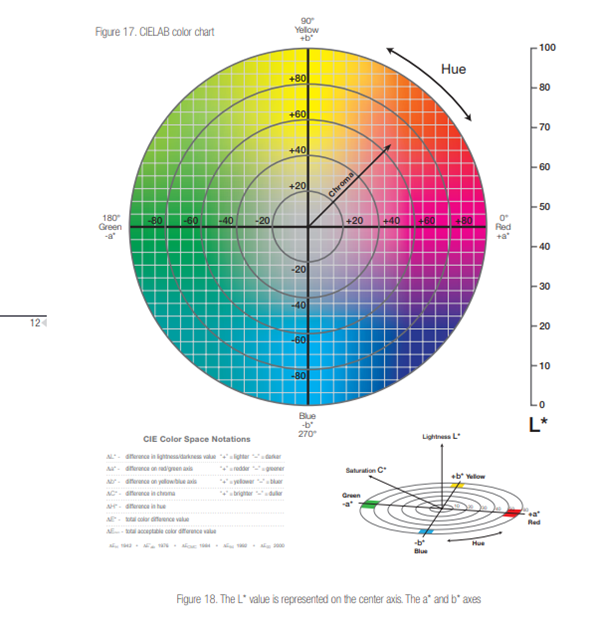
\includegraphics[scale=.55]{resources/colorspace/lab-color-space.png}}
  \caption{CIELAB Farbraum}
\end{figure}

\section{Neuronale Netzwerke}


\subsection{Aktivierungsfunktionen}
\subsection{Fully-Connected Neuronal Network}
\subsection{Convolutional Neuronal Network}
\subsection{Andere Layers}
\subsection{Kostenfunktionen}
\subsection{Backpropagation}
\subsection{Optimierungsalgorithmen}
% Beispiel Abbildung \ref{img:cnn_example_network} mit Zitat. \begin{figure}[H] \centering
% 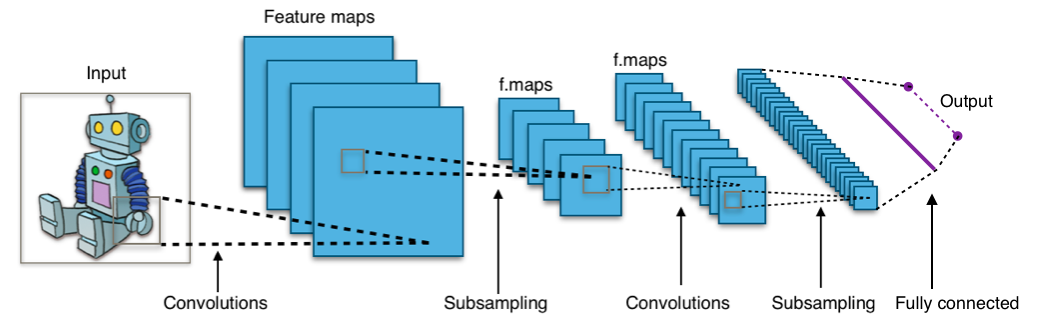
\includegraphics[width=0.95\textwidth]{resources/cnn/typical_cnn} \caption{Beispiel CNN Arhcitektur \cite{typical_cnn_img}}
% \label{img:cnn_example_network} \end{figure}
\section{Verwandte Arbeiten}
TODO